\documentclass{article} % set_input_method
\usepackage{hyperref}
\usepackage{graphicx}        % standard LaTeX graphics tool
\usepackage{enumitem}
\usepackage{xspace}
\newcommand{\ebop}[1]{\textrm{\bfseries #1}}

\newcommand{\eb}{\textsf{Event-B}\xspace}
\newcommand{\jml}{\textsf{JML}\xspace}
\newcommand{\ebtj}{\textsf{Event\-B\-2\-Java}\xspace}
\newcommand{\javacode}[1]{\texttt{#1}}

\usepackage{amssymb}
\usepackage[utf8]{inputenc}
\newcommand{\continuation}{\rotatebox[origin=c]{90}{$\curvearrowleft$}}
\newcommand{\continuationR}{\rotatebox[origin=c]{-90}{$\curvearrowright$}}

\newcommand{\lcb}{{\tt {\char '173}}}
\newcommand{\rcb}{{\tt {\char '175}}}

\usepackage{xcolor}

\definecolor{darkgreen}{rgb}{0,0.6,0}
\definecolor{darkblue}{rgb}{0,0,0.55}
\definecolor{darkred}{rgb}{0.4,0.0,0}
\definecolor{darkgray}{rgb}{0.66,0.66,0.66}
\definecolor{darkpink}{rgb}{0.91, 0.33, 0.5}
\definecolor{lightgray}{rgb}{0.95,0.95,0.92}
\definecolor{darkpurple}{rgb}{0.59, 0.44, 0.84}

\definecolor{pred}{rgb}{0.6,0,0}
\definecolor{pgrey}{rgb}{0.75,0.75,0.75}

\newcommand{\ebkeyw}[1]{\textcolor{pred}{\textsf{#1}}}
\newcommand{\ebtag}[1]{\textcolor{pgrey}{\textsf{\bf #1}}}
\newcommand{\ebcmt}[1]{\textcolor{pgrey}{\textsf{\it #1}}}
\newcommand{\ebcode}[1]{\textsf{#1}}
\newcommand{\ebsets}[1]{\textcolor{darkgreen}{\textsf{#1}}}
\newcommand{\ebcons}[1]{\textcolor{darkblue}{\textsf{#1}}}

 \oddsidemargin 0pt % -10.4mm
 \evensidemargin 0pt % -10.4mm
 % \marginparwidth 0pts
 \marginparsep 0pt
 \topmargin 0mm % -10.4mm
 \headheight 0pt
 \headsep 0pt
 \textheight 232mm % 257.2mm
 \textwidth 165mm % 169.2mm
 \footskip 25pt %


\begin{document}

\begin{center}
\rule{\textwidth}{.0075in} \\
\rule[3mm]{\textwidth}{.0075in}\\

Universidade do Algarve\hfill Parallel and Distributed Systems \hfill 2026\\[3ex]

{\Large\bf HW4 \\ \medskip Testing the Model of a Resilient Social Network} \\[3ex]

\vspace*{0.30cm} Nome: 
  \raisebox{.2ex}{\makebox[0pt][l]{}}{\line(1,0){260}} \ %
  \textnumero:\line(1,0){50}

\rule{\textwidth}{.0075in} \\
\rule[3mm]{\textwidth}{.0075in} \\
\end{center}

\bigskip

\noindent
\textbf{Goal.} The main goal of this lab is to unit test the resilient model that you developed in HW03. You use JUnit in Eclipse to unit test the cyber-resilient model for social networking that you developed in HW03. You are allowed to complete or edit the model you submitted for HW03.


\section{Pre-requisites}
\label{sec_pre}

\begin{enumerate}[leftmargin=*, label=(\textbf{\alph*}), itemsep=-5pt]
\item Make sure you successfully completed HW0, and you have installed all the required Rodin plugins.
  %
\item Read the document \texttt{docs/\-hw04\_\-doc01.\-pdf} that is included in this Overleaf project. This document shows how to install and use \ebtj and how to import the code generated by \ebtj in the Eclipse IDE. Make sure you have installed the Java version of Eclipse.
  %
\item Make sure you have carried out HW03. The \eb model produced in HW03 is the starting point of
  HW04. You are allowed to make corrections to the \eb model written during HW03, for instance, you
  can add events or remove existing events, you can redesign machines or contexts, or you can write
  a totally different model. It is all up to you.
  %
\item You will use Eclipse to manually write JUnit (Java Unit) tests for the Java code generated with
  \ebtj for the resilient model of social networking. Install JUnit in your Eclipse Java
  IDE. This link
  \href{https://www.qualitestgroup.com/insights/technical-hub/how-to-set-up-junit-in-eclipse/} {https://\-www.\-qualitest\-group.\-com/\-insights/\-technical-\-hub/\-how-\-to-\-set-\-up-\-junit-\-in-\-eclipse/}
  shows how to install JUnit in Eclipse.
  %
\item Read the document \texttt{docs/\-hw04\_\-doc02.\-pdf} that is included in this Overleaf
  project. It shows an example of how to unit test some of the functionality of a chat system.
  %
\item Optionally, you might want to import the file
  \texttt{docs/\-redes\_\-lab\-04\_\-PL1\_\-sol\-.zip} as a project in Eclipse to see what a JUnit
  Eclipse project looks like. Notice that this Eclipse project includes an \texttt{AllTests.java}
  file which is the main JUnit test oracle. Typically, you right-click on this file and then select
  \texttt{Run As}, then \texttt{JUnit Test}.
\end{enumerate}



\section{Steps}
\label{sec_steps}


\begin{enumerate}[leftmargin=*, label=(\textbf{\roman*}), itemsep=-5pt]
\item Use \ebtj to generate code for the last refinement (the most concrete machine) of your model
  for cyber-resilient social networks. You can reuse, adapt, or change your model in HW03, or you
  can just write a different model afresh. Make sure your model is sound and complete before
  proceeding further with this or the following steps.~\ebtj offers two alternatives for code
  generation, ``sequential'' or ``multi-threading''; make sure you select ``multi-threading'' when
  generating code with \ebtj.
%
\item In the previous step, \ebtj generated an Eclipse project in the form of a folder. In Eclipse,
  import the project (a zipped version of the folder). 
%
\item Still in Eclipse, write the JUnit tests stated in Section~\ref{sec_junit}. You are allowed to write one or several JUnit classes but you must include an \texttt{AllTests.\-java} test oracle that references any individual test classes that you write. \texttt{AllTests.\-java} is the only test file that will be run to evaluate and grade your work.
%  
\item All the JUnit tests that you write are expected to pass. However, if a test does not pass, you might either revisit the code of the JUnit test or revisit your \eb model and generate code again. You are allowed to write JUnit tests but you are not allowed to edit the code generated by \ebtj. Doing so will be to the detriment of your grade.
%
\end{enumerate}
\section{JUnit tests}
\label{sec_junit}

Figure~\ref{fig_test01} presents an example of a JUnit test: the system can send a ping right after it is created, but it cannot send a second ping immediately after the first ping (that is, before an echo occurs). \ebtj generates a Java class for each event. This class includes a ``guard'' and ``run'' method. For instance, the \texttt{send} class includes a \texttt{guard\_send} boolean method that evaluates the event guard, and a \texttt{run\_send} method that executes the \ebcode{send} event. For the purposes of this homework assignment, you should name your unit tests methods as \texttt{test\_\-01()}, \texttt{test\_\-02()}, and so on. Notice that this and other JUnit tests can look different for you depending on how your \eb model works.

In the following, we assume that the event that pings the server is called \ebcode{send}, and the event that performs echo is called \ebcode{receive}. We assume the existence of an event \ebcode{hasFailed} that is enabled whenever the system is in a failed state, and an event \ebcode{fail} that put the system into a failed state. Furthermore, the event \ebcode{send} is ``disabled'' means ``its guard does not hold''. The event \ebcode{send} is ``enabled'' means ``its guard holds''.

Next, we state the JUnit tests that you should include in your homework. The JUnit tests must be written in  Eclipse.


\begin{figure}
\centering 
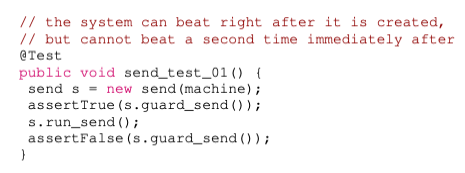
\includegraphics[width=10cm]{./figs/test01.png}
\caption{JUnit test example}
\label{fig_test01}
\end{figure}


\subsection*{Part I}

The following tests assume a sole client who can ping a sole server, and the same server who can echo the ping. Consequently, \ebcode{hasFailed} means ``the communication between the sole client and the sole server \ebcode{hasFailed}'', \ebcode{fail} refers to an event that causes the communication between a client and a single server to \ebcode{fail}, etc.

\begin{enumerate}[leftmargin=*, label=(\textbf{\arabic*})]
  %
\item after \ebcode{send} is executed, \ebcode{send} is always disabled, unless
  \ebcode{rollback} or \ebcode{receive} are executed (\texttt{test\_\-01()}).
  %
\item after \ebcode{send} is executed, \ebcode{receive} is always enabled, unless
  \ebcode{fail} is executed (\texttt{test\_\-02()}).
  %
\item after \ebcode{fail} is executed, \ebcode{hasFailed} is always enabled, unless
  \ebcode{rollback} is executed (\texttt{test\_\-03()}). 
  %
\item after \ebcode{hasFailed} is enabled, \ebcode{rollback} is always enabled (\texttt{test\_\-04()}). 
  %
\item after \ebcode{hasFailed} is enabled, \ebcode{send} is always disabled, unless
  \ebcode{rollback} is executed (\texttt{test\_\-05()}).
  %
\item after \ebcode{hasFailed} is enabled, \ebcode{receive} is always disabled, unless
  \ebcode{send} is executed (\texttt{test\_\-06()}). 
  %
\item after \ebcode{fail} is executed, \ebcode{rollback} is always enabled, unless
  \ebcode{rollback} is executed (\texttt{test\_\-07()}). 
\end{enumerate}


\subsection*{Part II}

In the following, we say that ``A does not affect or does not
influence B'' if the success or failure of B does not depend on the
success or failure of A. Therefore, B will succeed regardless of the
success or failure of A. We say that a ping times-out when it is not
followed by an echo within a time limit.

\begin{enumerate}[leftmargin=*, label=(\textbf{\arabic*})]
\item a client can ping 3 (or more) different servers; each server is able to echo its respective
  ping; and, a server echoing a ping does not affect the ``enabledness'' of the rest of pings
  (\texttt{test\_\-08()}).
  %
\item a client can ping 3 (or more) different servers; each of the pings can timeout independently,
  hence, the timeout of any of the pings is not influenced by the timeouts of the other 2 pings
  (\texttt{test\_\-09()}).
  %
\item a client can ping 3 (or more) different servers and each ping times-out independently; if the
  3 pings timeout, the ability of any of the servers to recover (rollback) does not influence the
  ability of any of the other two servers to recover (\texttt{test\_\-10()}).
  %  
\end{enumerate}


\section{Grading criteria}


\begin{enumerate}[leftmargin=*, label=(\textbf{\alph*}), itemsep=-5pt]
\item \textbf{Completeness.}~Your \eb model includes the most relevant functionality of a cyber-resilient system, including, ping, echo, failures, timeouts, rollbacks, several clients, several servers.
  \item \textbf{Soundness.}~All proof obligations of the \eb model are discharged.
  \item \textbf{Adequacy.}~Your model represents the functionality of a cyber-resilient
    client-server system in which several clients and several servers intervene.
  \item \textbf{Simplicity.}~The \eb model is well-structured, readable without unnecessary complexity. 
  \item \textbf{Originality.}~This is your own work, not the work of others. 
  \item \textbf{Novelty.}~Your solution demonstrates original ideas. 
  \item \textbf{Correctness and validation.}~The Java implementation behaves as expected in JUnit testing scenarios, providing evidence that the model captures the intended behaviour.
\end{enumerate}

\section*{What should you turn in?}
\label{sec_what_to_turnin}

You must submit $(i.)$ a ZIP file with your Rodin project, and $(ii.)$ a ZIP file with your
Eclipse project that includes the JUnit tests (right-click the project then select \texttt{Export},
\texttt{General}, \texttt{Archive File}).~\\

\smallskip
%
  \textcolor{red}{I reserve the right to single you out and ask you to
    personally demonstrate (validate) your work orally or in
    writing}. \textcolor{red}{I also reserve the right to ask you for
    further information about your work after you submit it}.


\end{document}
